\documentclass{standalone}
\usepackage{float}
\usepackage{graphicx}
\usepackage{tikz}

\colorlet{headingbg}{black!5}

% Set styles for TikZ objects
\usetikzlibrary{angles, arrows, calc, circuits.ee.IEC, decorations.markings,
    decorations.pathreplacing, patterns, positioning, quotes, shapes}
\tikzstyle{block} = [draw, fill=headingbg, rectangle, minimum height=3em,
    minimum width=4em]
\tikzstyle{sum} = [draw, circle, node distance=1cm]
\tikzstyle{arrow} = [arrows=->, black, align=right]
\tikzstyle{branch} = [circle, inner sep=0pt, minimum size=1mm, fill=black,
    draw=black]
\tikzstyle{opencircuit} = [circle, draw=black, fill=white, minimum size=3pt,
    inner sep=0pt]

\begin{document}
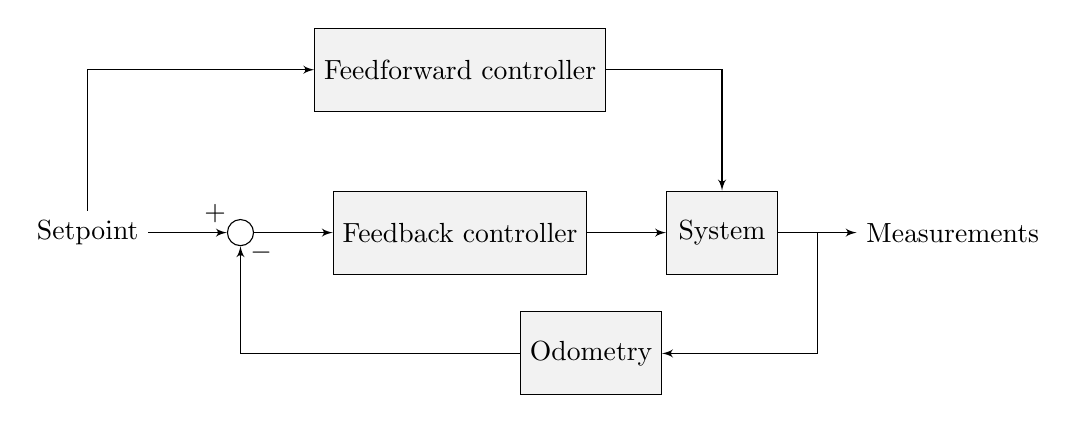
\begin{tikzpicture}[auto, >=latex']
  % Place the blocks
  \node [name=input] {Setpoint};
  \node [sum, right=of input] (sum) {};
  \node [block, right=of sum] (K) {Feedback controller};
  \node [block, above=of K] (Kff) {Feedforward controller};
  \node [block, right=of K] (G) {System};
  \node [right=of G] (output) {Measurements};
  \node [block, below=of $(K)!0.5!(G)$] (H) {Odometry};

  % Connect the nodes
  \draw [arrow] (input) -- node[pos=0.85] {$+$} (sum);
  \draw [arrow] (sum) -- node {} (K);
  \draw [arrow] (input) |- node {} (Kff);
  \draw [arrow] (Kff) -| node {} (G);
  \draw [arrow] (K) -- node {} (G);
  \draw [arrow] (G) -- node[name=y] {} (output);
  \draw [arrow] (y) |- (H);
  \draw [arrow] (H) -| node[pos=0.97, right] {$-$} (sum);
\end{tikzpicture}
\end{document}
